\begin{figure*}[t]
  \centering
  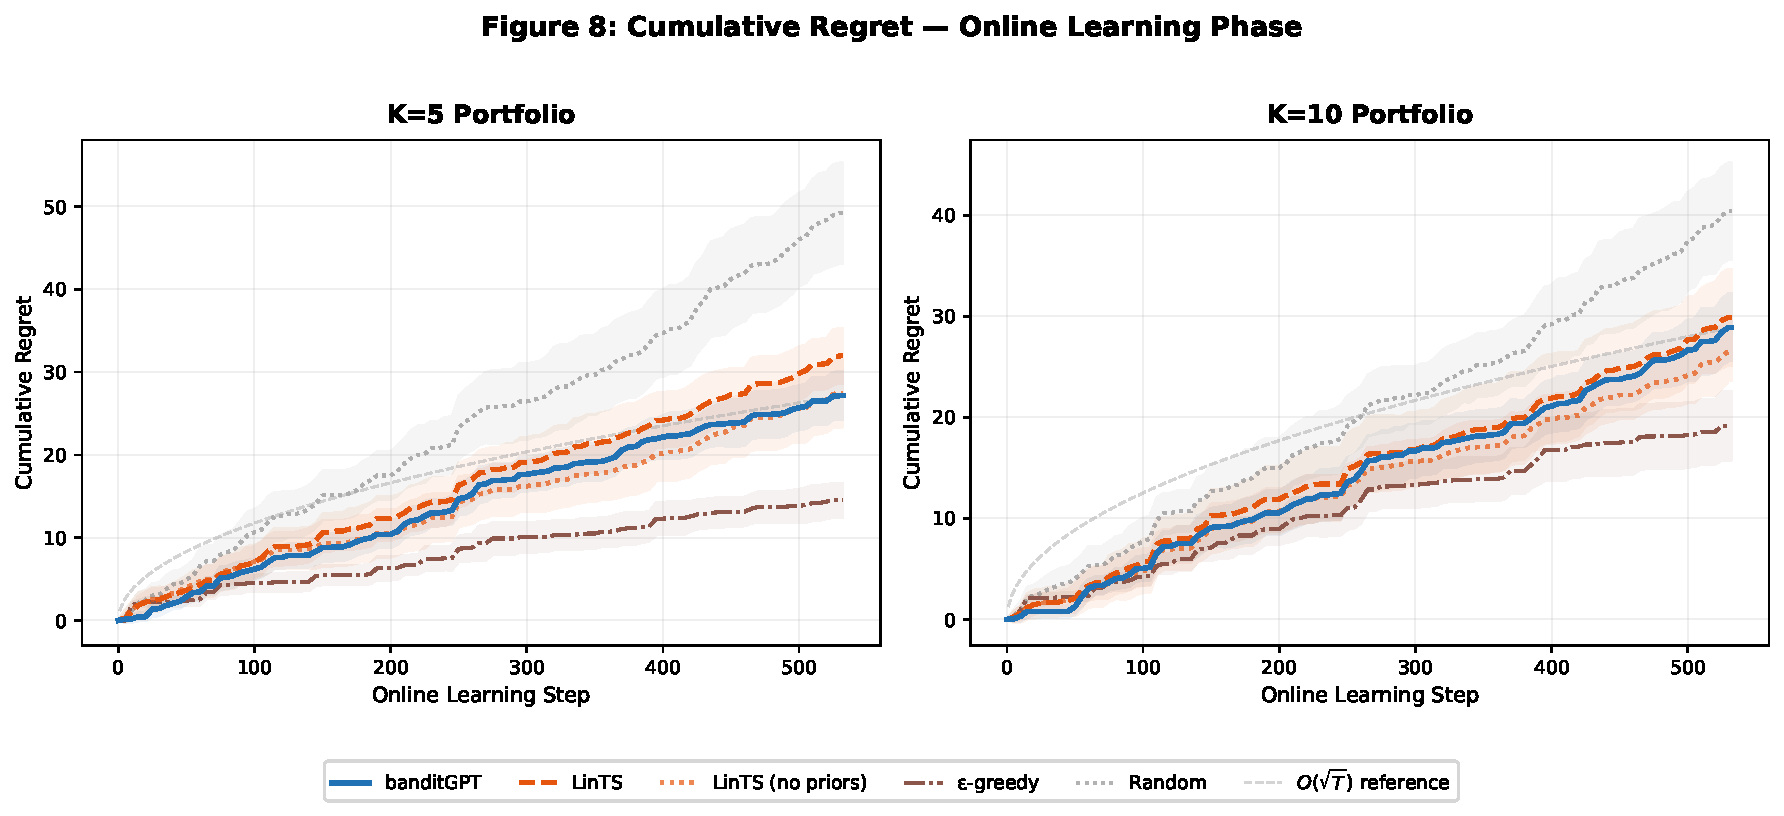
\includegraphics[width=\textwidth]{../experiments/08_figure/results/figure8_cumulative_regret.pdf}
  \caption{
    \textbf{Cumulative Regret During Online Learning ($K{=}5$, $K{=}10$).}
    Among contextual bandits, banditGPT achieves the lowest regret at $K{=}5$ (27.1 vs.\ 31.9 for LinTS, $-15\%$) and is competitive at $K{=}10$ (28.9 vs.\ 29.9).
    Both contextual methods track below the $O(\sqrt{T})$ reference (grey dashed), confirming theoretical sub-linear regret.
    $\varepsilon$-greedy achieves the lowest overall regret (14.5 at $K{=}5$) by exploiting the single best-on-average model (GPT-4.1).
    This is expected: when one model dominates (contextual ceiling $=1.7\%$), non-contextual methods benefit from a favourable $O(K/\Delta \log T)$ bound, whereas contextual methods incur $O(d\sqrt{KT})$ exploration costs.
    The value of contextual routing emerges at nonzero cost penalties (Section~\ref{sec:egreedy_analysis}), where the oracle routes $74.5\%$ of traffic to the $136\times$ cheaper Llama-3.1-8B.
    Shaded bands: $\pm 1\sigma$ across 20 trials.
  }
  \label{fig:cumulative_regret}
\end{figure*}
